\section{Fundamentals of blockchain}\label{sec:fundamentals}
In this section, the key elements of the blockchain that contribute to its properties will be displayed: integrity, immutability, transparency, availability, disintermediation, decentralization.

\subsection{Cryptography}\label{sec:criptografia}
Blockchain relies heavily on encryption to satisfy system and application security requirements. As the word suggests, cryptocurrencies also make heavy use of encryption. Encryption provides a mechanism for safely encoding the rules of a system encryption on the system itself. This can be used to prevent tampering and misconceptions, as well as coding in a mathematical protocol, the rules for creating new currency units. So, before be able to understand blockchains correctly, it is necessary to understand the cryptographic foundations they trust \cite{narayanan2016bitcoin}.

Cryptography is a deep academic field of research that uses many advanced mathematical techniques that are notoriously subtle and complicated. In this chapter, cryptographic hashes and digital signatures will be defined, which stand out among the most used resources. For more details, the reader should refer to the book \cite{narayanan2016bitcoin}.

\subsubsection{Cryptographic Hashes}\label{sec:hashesCriptograficos}
A hash function is a mathematical function with the three properties to be follow \cite{narayanan2016bitcoin}:

\begin{itemize}
\item  Its input can be any string of any length;
\item Produces a fixed size output. For the purpose of making concrete
the discussion in this chapter (eg., 256 digits);
\item It is efficiently computable. Intuitively, this means that for
a given input string, is possible to find out what is the hash function output within a reasonable period of time. Technically, hashing a n-bit string must have a $O(n)$ runtime.
\end{itemize}

These properties define a general hash function. Cryptographic hash functions (or cryptographic summaries) are unidirectional and hardly allow retrieving the original value $x$ from the hash $h$. For a hash function to be cryptographically secure, it must satisfy the following three properties: (1) collision resistance, (2) hiding and (3) puzzle friendliness \cite{greve2018blockchain}.

A collision occurs when two distinct inputs produce the same output. A hash function $H$ is collision resistant when it is impossible to find two values $x$ and $y$ such that $x \neq y$ and $H(x) = H(y)$ \cite{narayanan2016bitcoin}.

The hide property states that, having the hash function output $y = H (x)$, there is no possible way to find out which whas the $x$ input \cite{greve2018blockchain}.

A hash function $H$ is considered puzzle friendliness if for each possible output value of $n$ bits $y$ if $k$ is chosen from a distribution with high min-entropy, then it is impracticable to find $x$ such that $H (k \| x) = y$ in time significantly less than $2^n$ \cite{narayanan2016bitcoin}.

\subsubsection{Digital Signatures}\label{sec:assinaturasDigitais}
A digital signature is supposed to be a digital analog of a handwritten paper signature. Two signature properties are desired which correspond well to the analogy of the handwritten signature: first, only one person can make their own signature, but anyone can verify if it is valid. Secondly, it is desired that the signature must be linked to a specific document, so the signature cannot be used to indicate the agreement or endorsement to a different document \cite{merkle1989certified}. Moreover, it is not possible to forge a signature in such a way as to reuse it in some other context. That is, signatures must be irrefutable.

To implement digital signatures, asymmetric key encryption is used. A secret key (sk) is used for signing the document and a public key (pk) is used to attest the signature's authenticity \cite{greve2018blockchain}.

A digital signature consists of the following three algorithms \cite{narayanan2016bitcoin}:

\begin{itemize}
\item $(sk , pk) := generateKeys(keysize)$ – The $generateKeys()$ method receives a key size $(keysize)$ in the input and return a pair of public $(pk)$ and private $(sk)$ keys.
\item $sig := sign(sk , msg)$ – The method $sign()$ receives a message $msg$ and a secret key $(sk)$ on entry and returns the signature $sig$ f that message under $sk$.
\item $isValid := veri f y(pk , msg , sig)$ – The method $verify$ receives a public key $(pk)$, a message $msg$ and a signature $(sig)$ as input, and returns a boolean value: $isValid = true$ if $sig$ is a signature valid for $msg$ under $pk$; $isValid = false$, otherwise.
\end{itemize}

The following two properties must be maintained:

\begin{itemize}
\item Authenticity: Signatures can be validated: \\ $verify(pk, message, sign(sk, message)) = = true$.
\item Signatures are existentially unfalsifiable: signature cannot be forged.
\end{itemize}

It is noted that generateKeys() and sign() can be random algorithms. In fact, generating keys should be randomized, because it should be generating different keys for different people. On the other hand, verify() will always be deterministic.

\subsection{Consensus}\label{sec:consenso}
The key to blockchain operation is that the network must agree collectively on the ledger's content. Instead of a central entity maintain control over information (such as a bank for example), the data is shared among all. This requires the network to maintain the consensus around the information recorded in the block chain. How this consensus is reached, affects the security and economic parameters of the protocol \cite{kostarev2017review}.

In this context, consensus emerges as a fundamental problem, since it allow distributed participants to coordinate their actions in order to reach common decisions, thereby ensuring the consistency of safety and system progress (liveness) despite the existence of of failures \cite{greve2018blockchain}. More specifically, in the context of blockchain, consensus enables to reach agreement on the next block that will be added to the blockchain.

In blockchain, reaching consensus between untrusted nodes is a transformation of the problem of \ac{BG} \cite{lamport1982byzantine}. In the BG problem, a group of generals who command a portion of the Byzantine army circles the city. The attack would fail if only part of the generals attacked the city. Generals need to communicate to agree on the attack or not. However, there may be traitors in the generals. The traitor could send different decisions to different generals. This is an environment without trust.

Reaching consensus in such an environment is a challenge. This is also a challenge for blockchain, because its network is distributed and there is no central node that ensures that ledgers on distributed nodes be all the same. Nodes do not need to trust other nodes. Thus, some protocols are required to ensure that ledgers on different nodes are consistent \cite{kostarev2017review}. To solve the consensus problem, several algorithms have been proposed and are listed below. For more details on each algorithm is recommended to read the article \cite{mingxiao2017review}.

\begin{itemize}
\item Proof-of-Work;
\item Proof-of-Stake;
\item Delegated Proof-of-Stake;
\item Leased Proof-Of-Stake;
\item Proof of Elapsed Time;
\item Practical Byzantine Fault Tolerance;
\item Simplified Byzantine Fault Tolerance;
\item Delegated Byzantine Fault Tolerance;
\item Directed Acyclic Graphs;
\item Proof-of-Activity;
\item Proof-of-Importance;
\item Proof-of-Capacity;
\item Proof-of-Burn;
\item Proof-of-Weight;
\end{itemize}

A good consensus algorithm means efficiency, security and convenience. Current common consensus algorithms still have many shortcomings. New consensus algorithms are created to solve some blockchain-specific problems \cite{zheng2016blockchain}.

\subsection{Distributed Ledger}\label{sec:livro}
Distributed ledger is a data structure distributed by several nodes or computing devices. Each node replicates and saves a identical ledger copy. Each participating node in the network updates independently \cite{greve2018blockchain}.

The innovative feature of distributed accounting technology is that the ledger is not maintained by any central authority. Updates to The ledger are independently constructed and recorded by each node. The nodes then vote on these updates to ensure that most agree with the conclusion reached, based on some previous consensus algorithm. Once consensus has been reached, the distributed ledger updates itself and the latest agreed version is saved on each separate node \cite{swan2015blockchain}. Thus, the distributed ledger is replicated and immutable. 

\subsubsection{Transactions}\label{sec:transac}
The blockchain is a public digital book that records online transactions. In it, transactions are recorded in a block without the help of third parties, such as a bank or payment processor. The blockchain algorithm automatically graphs and authenticates the transaction, which is immediately visible to all users, minimizing the possibility of fraud. The terms of transaction do not include any personal or identifying information \cite{Bankrate2018}.

From a technical standpoint, the most fundamental definition of a transaction is an atomic event allowed by the underlying protocol. A transaction determines a sequence of state operations. It adds a transfer of asset or, generally speaking, a smart contract. In a basic case, the transaction girds a digital signature of the issuer holding the asset and the receiver's address, as well as inputs and outputs for transaction. Each transaction must contain both Inputs and Outputs just like in a accounting book. Entries indicate the previous transaction hash which is related to the current one \cite{greve2018blockchain}. Validating a Transition involves:

\begin{enumerate}
	\item signature verification;
	\item confirmation of existing values from hashes of previous referenced transactions;
	\item confirmation that the amount was not previously spent by any other transactions.
\end{enumerate}

In this case, it is necessary to search the blockchain between the block from the referenced transaction to the last block of the structure. Transactions are independently validated by each node of the blockchain network, and this feature contributes to the decentralization of the process \cite{greve2018blockchain}.

\subsubsection{blocks}\label{sec:blocks}
Blocks contains a header with information needed for current maintenance and its validation. A block consists of the block header and block body as shown in Figure \ref{fig:block}. 

\begin{figure}[htbp]
\begin{center}
  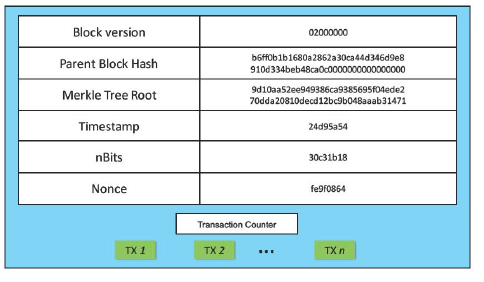
\includegraphics[scale=0.5]{images/blockStructure.png}
\caption{Structure of a block. \cite{zheng2016blockchain}}
\label{fig:block}
\end{center}
\end{figure}

In particular, the header Pack includes:

\begin{itemize}
\item Block version: indicates which set of block validation rules to follow..
\item Parent block hash: A 256-bit hash value that points to the previous block.
\item Merkle tree root hash: The hash value of all transactions in the block.
\item Timestamp: Current date and time as seconds since 1970-01-01T00:00 UTC.
\item  nBits: current hashing target in a compact format.
\item Nonce: A 4-byte field, usually starting with 0 and increasing for each hash.
\end{itemize}

The body's block consists of a transaction counter and transaction. The maximum number of transactions a block can hold depends on block size and the size of each transaction. Blockchain uses a asymmetric encryption mechanism to validate transaction authentication. A digital signature based on asymmetric encryption is used in an untrusted environment \cite{zheng2016blockchain}.

The validation of a block consists in verifying (i) if its structure is well formed (ii) its hash is valid (meets the challenge), (iii) its size is within the network accepted limit, (iv) the set of transactions within the block is valid, (v) the first transaction (and only the first) is the coinbase transaction - which incorporates the generation of new cryptocurrencies in the system, besides acting as a reward mechanism. The blocks are validated independently, by each node of the blockchain network, and this feature contributes to the process decentralization \cite{greve2018blockchain}.

In mining process, new transactions are vilified by the nodes in the whole system known as “miners” before being added to blockchain. Miners add new blocks on the chain or new transactions on the block by a consensus algorithm, which must be confirmed by majority or all the nodes in the system, like a voting operation, as the valid data. Blockchain-based systems rely on miners to aggregate transactions into blocks and append them to the blockchain. Once the transaction is confirmed by a sufficient number of nodes, it becomes a valid and permanent part of the database. The figure \ref{fig:blockchain} presents a visual representation of a blockchain \cite{tian2017supply}.

\begin{figure}[htbp]
\begin{center}
  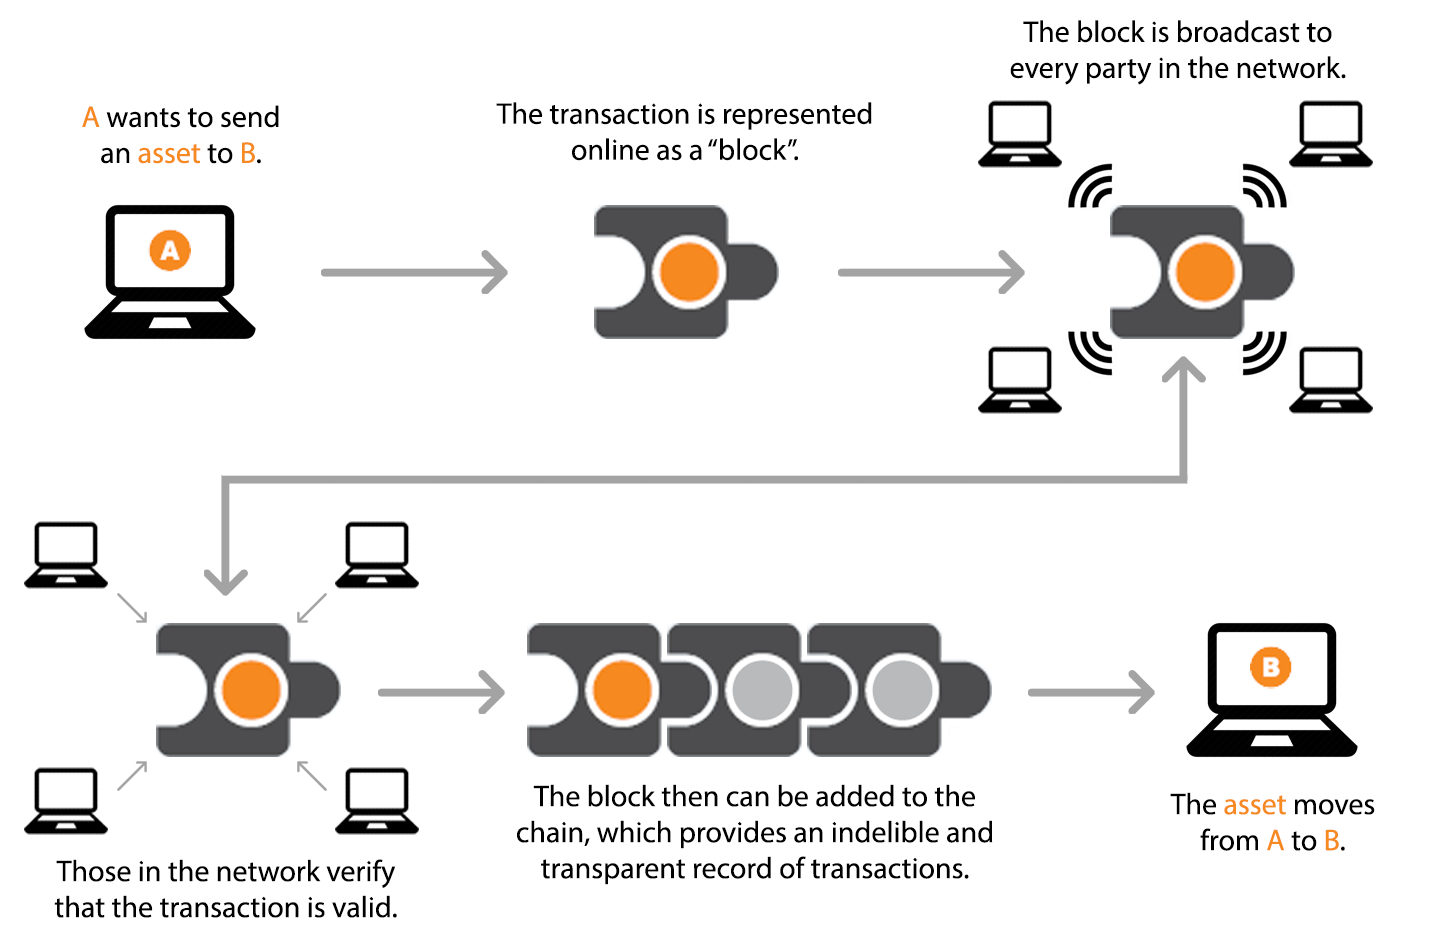
\includegraphics[scale=0.35]{images/blockchain.png}
\caption{Blockchain representation \cite{michael2018blockchain}}
\label{fig:blockchain}
\end{center}
\end{figure}
